% -*-mode: Latex-*-
% !TEX root = kampf.tex
% authors: simon maurer
%
% file: fkSF.tex
% contents: Sonderfertigkeiten für den Fernkampf
% Sccs-Id: %W% %G%

%==============================================================================

\section{Sonderfertigkeiten für den Fernkampf}
Folgende Abbildung gibt eine Übersicht über alle Sonderfertigkeiten (mit AP-Kosten und Voraussetzungen), die im Fernkampf eingesetzt werden können.
Es handelt sich dabei nicht um die Manöver. Diese werden im Kapitel 13 beschrieben.

\begin{figure}
    \centering
    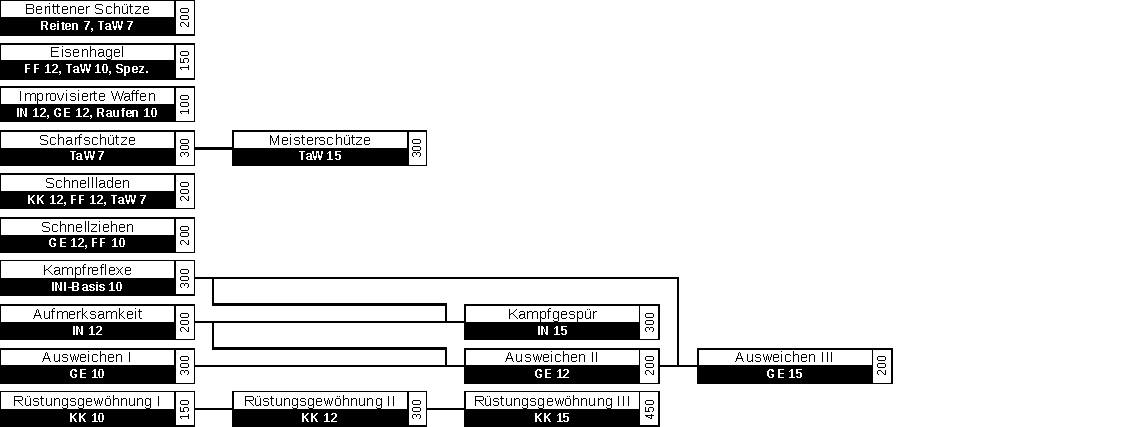
\includegraphics[width=16.93cm,height=6.454cm]{fkSF.pdf}
\end{figure}
